%* Source: https://tex.stackexchange.com/a/158979
\documentclass[tikz]{standalone}
\usepackage{pgfplots, calc, tkz-euclide}
\pgfplotsset{compat=1.18}
\usetikzlibrary{decorations.pathreplacing, decorations.markings, angles}

% axis style, ticks, etc
\pgfplotsset{every axis/.append style={
                    axis x line=middle,    % put the x axis in the middle
                    axis y line=middle,    % put the y axis in the middle
                    axis line style={->}, % arrows on the axis
                    }}

% arrows as stealth fighters
\tikzset{>=stealth,
-<-/.style={decoration={
  markings,
  mark=at position #1 with {\arrow[scale=1.5]{Classical TikZ Rightarrow[reversed]}}},postaction={decorate}}}
\NewDocumentCommand\bisector{O{}mmmO{10pt}}{
\path[#1] let
    \p1 = ($(#3)!10cm!(#2)$),
    \p2 = ($(#3)!10cm!(#4)$),
    \p3 = ($(\p1) + (\p2) - (#3)$)
    in    
    ($(#3)!#5!($(#3)!0.85cm!(\p3)$)$) -- ($($(#3)!0.85cm!(\p3)$)!#5!(#3)$) ;
}
\begin{document}

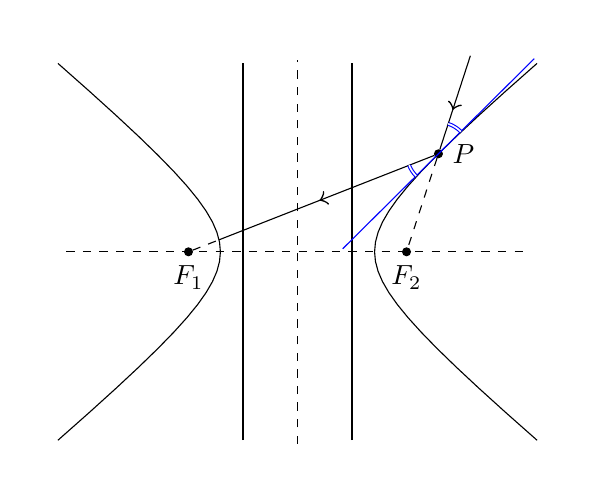
\begin{tikzpicture}[dot/.style={draw,fill,circle,inner sep=1pt}]
    \begin{axis}[
        xmin=-35,xmax=35,
        ymin=-35,ymax=35,
        axis line style={draw=none},
        ticks=none]
        % Hyperbola
        \addplot [domain=-1.8:1.8] ({10*cosh(x)}, {10*sinh(x)});
        \addplot [domain=-1.8:1.8] ({-10*cosh(x)}, {10*sinh(x)});
        % Asymptotes
        % \addplot[dashed,domain=-10*cosh(1.8):10*cosh(1.8)] expression {x};
        % \addplot[dashed,domain=-10*cosh(1.8):10*cosh(1.8)] expression {-x};
        % \coordinate[label={below left:\(O\)}] (O) at (axis cs:0,0);
        % focal points
        \node[dot,label={below:$F_1$}] (F1) at (axis cs:-14.14213562,0) {};
        \node[dot,label={below:$F_2$}] (F2) at (axis cs: 14.14213562,0) {};
        % node on hyperbola
        \node[dot,label={right:\(P\)}] (X) at (axis cs: 18.2843,15.3073) {};
        % path of light ray
        \coordinate (Y) at (axis cs:-10.1739,1.8732) {};
        \coordinate (Z) at (axis cs:22.4265,30.6149) {};
        \draw[-<-=.5] (Y) -- (X);
        \draw[dashed] (F1) -- (Y);
        \draw[dashed] (X) -- (F2);
        \draw[-<-=.5] (X) -- (Z);

        % Lines of symmetry
        \draw[dashed] (axis cs:-30,0) -- (axis cs:30,0);
        \draw[dashed] (axis cs:0,-30) -- (axis cs:0,30);
        % directrices
        \draw (axis cs:-7.071067812,-29.421742881) -- (axis cs:-7.071067812,29.421742881);
        \draw (axis cs:7.071067812,-29.421742881) -- (axis cs:7.071067812,29.421742881);
        \coordinate (D1) at (axis cs:-9.071067812,-29.421742881);
        \coordinate (D2) at (axis cs:8.071067812,-29.421742881);
        % tangent point
        \node (K) at (axis cs: 10,5.412) {};
    \end{axis}
    % Tangent and angle
    \draw[blue] ($(X)!-1.5!(K)$) coordinate (U) --($(X)!+1.5!(K)$) coordinate (V)
        pic [draw,blue,double,angle radius=0.4cm] {angle = U--X--Z}
        pic [draw,blue,double,angle radius=0.4cm] {angle = F1--X--V};
\end{tikzpicture}

\end{document}